\chapter{Rezumatul proiectului}

Proiectul 4.5G își propune implementarea unei punți între tehnologiile
curente 4G și cele emergente 5G. Această punte se realizează la
nivelul transport (TCP) prin folosirea noului protocol de transport
MPTCP pentru a utiliza în mod transparent, cumulativ si simultan
tehnologiile de rețea existente, în principal 3G/4G și WiFi, dar
potențial și alte tehnologii de comunicatie disponibile pe mobile în
viitor.


Scopul proiectului este de a instrumenta terminale Android existente,
astfel încât upgrade-ul la MPTCP nu aduce un regres de uzabilitate sau
necesitatea recompilării aplicațiilor. Avantajele aduse sunt {\bf
  conectivitatea continuă} la schimbarea rețelei WiFi sau 4G, {\bf
  capacitatea crescută} când ambele rețele sunt prezente, și {\bf
  viteză ridicată de răspuns} pentru aplicațiile interactive.


\section{ Nivel de maturitate al tehnologiilor (Tehnology Readiness Levels)}

Proiectul a demarat la nivelul TRL2, avănd beneficii clare pentru
operatori și utilizatori finali, si o literatură de specialitate care
include experimente incipiente, implementări propuse, și unele măsurători. 

Pe parcursul proiectului, mai multe etape specifice TRL3 au fost
atinse - mai multe arhitecturi de proxy au fost evaluate analitic si
experimental, arhitectura aleasă implicând folosirea RTT (round trip
time) care afectează utilizatorii.  

Livrabilul final al proiectului este un demonstrator situat la nivelul
TRL4: un telefon instrumentat și serverul proxy asociat de plasat la
operatorul 4G au fost testate într-un mnediu controlat dar realistic
la partenerul Orange Romania. Componentele au fost validate prin teste
în rețeaua 4G și WiFi, și prototipul este valid ca funcționalitate și
performanță.

\pagebreak

\section{Imagini reprezentative}

\begin{figure}[h]
	\centering
	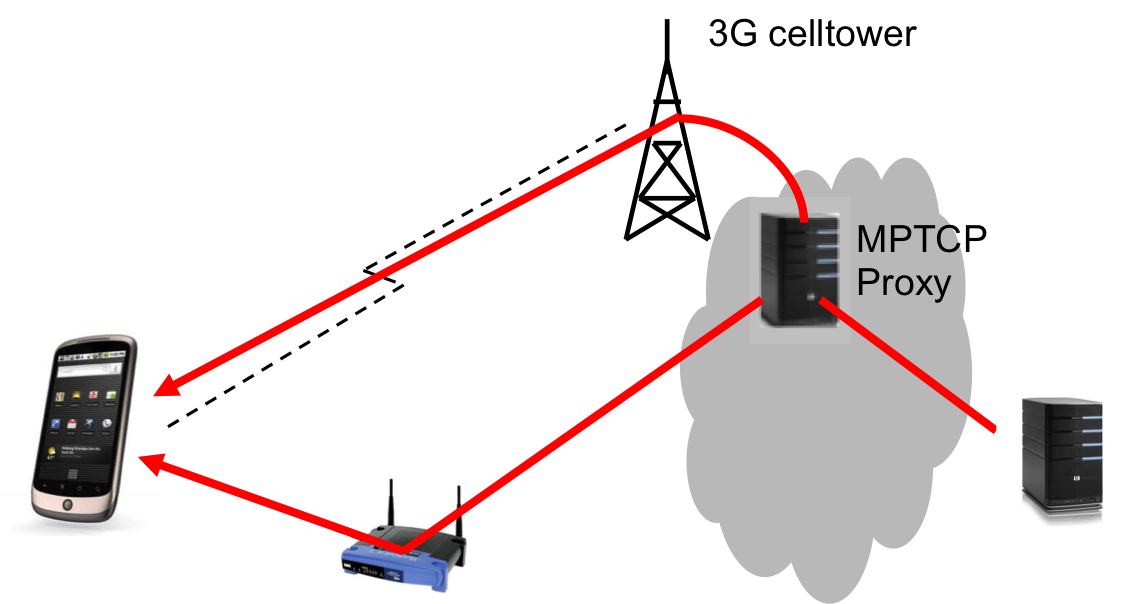
\includegraphics[scale=0.7]{figures/45g_proxy.png}
	\caption{Comunicația prin proxy}
\end{figure}


%% \begin{figure}[h]
%% 	\centering
%% 	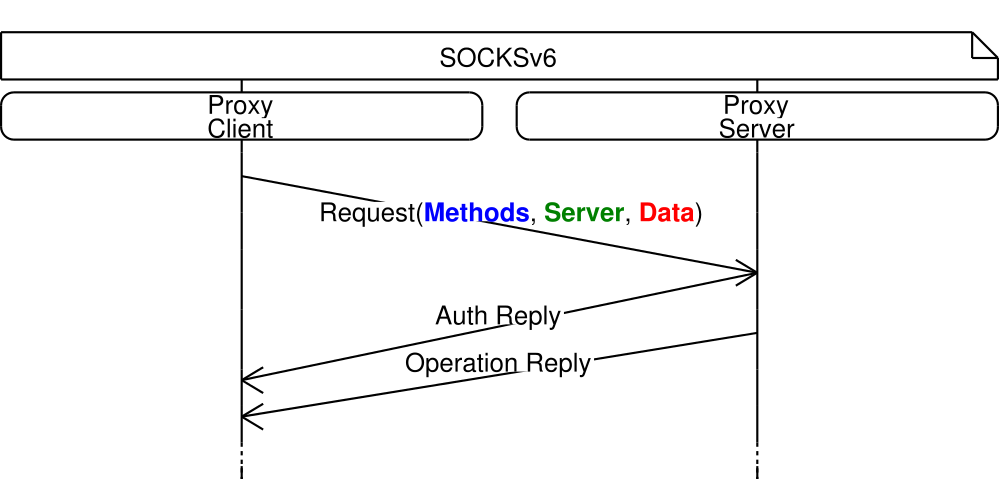
\includegraphics[scale=0.7]{figures/socks/socks6op2nd.png}
%% 	\caption{Mod de operare SOCKS 6 (conexiuni ulterioare)}
%% \end{figure}

\begin{figure}[h]
        \centering
        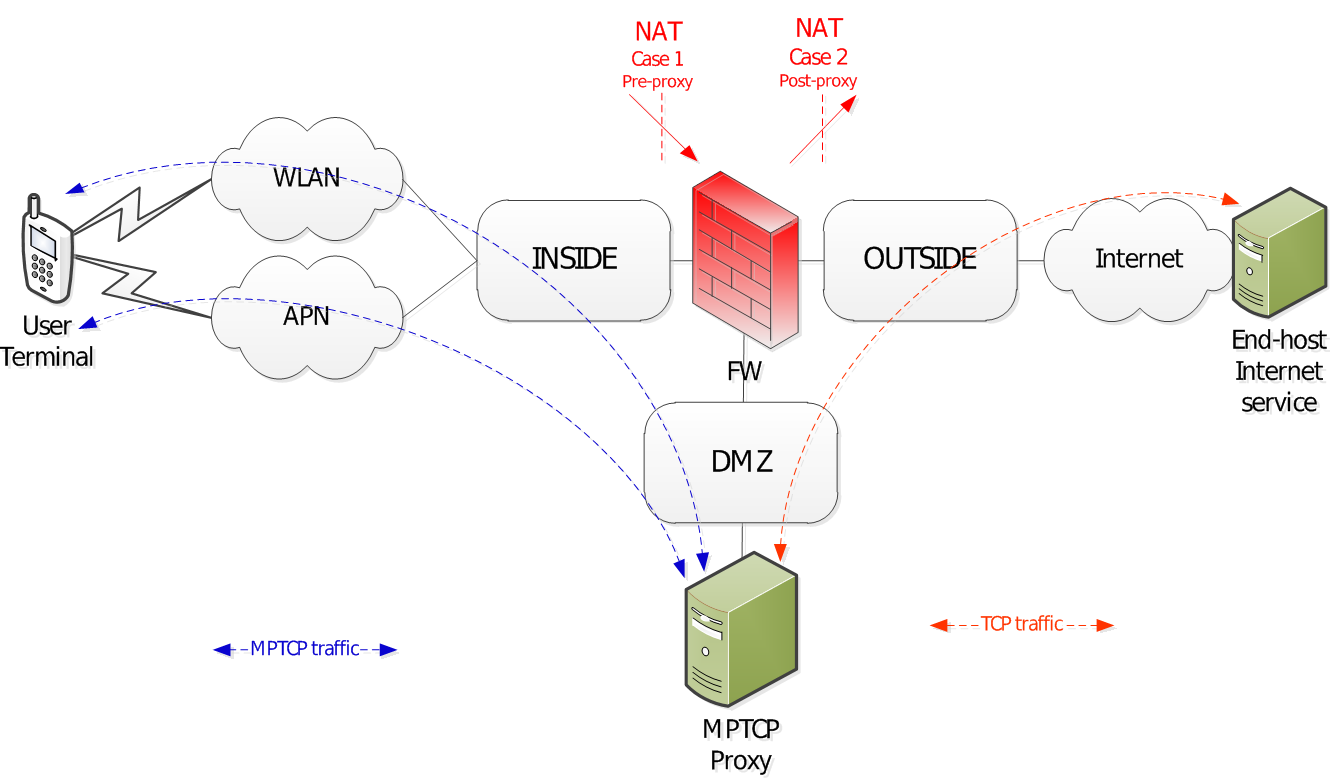
\includegraphics[scale=0.3]{figures/oro/oro_mptcp.png}
        \caption{Plasarea proxy-ului de MPTCP în rețeaua Orange Romania}
\end{figure}


 
